\ssection{Drive do GECOM}
	Para facilitar o acesso dos alunos do curso de eletrônica à informação, o GECOM (Grêmio de Eletrônica e de Computação) criou uma pasta compartilhada no \textit{Google Drive}. Nessa pasta podemos encontrar:

	\begin{itemize}
        \item PDFs de materiais
        \item Provas antigas
        \item Exercícios
        \item Apresentações de slides/conteúdos dados em aula
	\end{itemize}
	
	Nosso drive é super organizado: lá você pode encontrar o material que deseja facilmente, já que existe uma pasta para cada disciplina. 

	Para acessar o drive, basta clicar nesse link enquanto logado com conta do PoliMail (domain @poli.ufrj.br): 
    \begin{center}
    	\href{http://bit.ly/2TciLzG}{Link do Drive}
   	\end{center}

	Se você ainda não tem conta na poli, aguarde a criação. Geralmente não demora muito: na primeira ou segunda semana de aula vocês já terão as suas contas ativadas! A escolha do endereço de e-mail é feita no dia de inscrição de disciplinas.
    
    Sei que você deve estar se perguntando "Mas como vocês conseguiram centralizar tanto material importante?"  E a resposta é: o drive da Eletrônica é atualizado por meio de contribuições dos próprios alunos do curso. 
    
    Todos nós, veteranos, entendemos a importância que o drive tem no nosso dia-a-dia. Por isso, sempre que possível, é uma boa prática contribuir com materiais atualizados (sejam provas, projetos ou material usado em aula).
    
    \textbf{Devemos deixar claro que é explicitamente proibido compartilhar materiais com direitos autoriais no Drive, como livros.} Além disso, todo o material a ser disponibilizado no Drive precisa ter sua divulgação previamente aceita pelo professor que possui os direitos do material.
    
    Uma vez que tais requisitos acima foram satisfeitos, basta seguir os seguintes passos:
    
    1) Clicar na pasta \textit{New}
    \begin{center}
		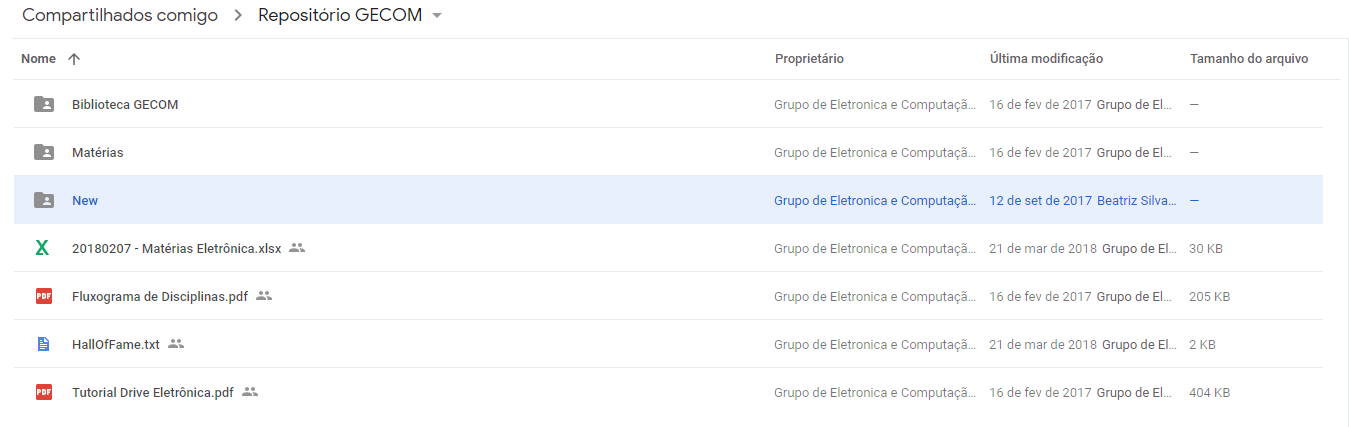
\includegraphics[width=\textwidth]{assets/driveGecomEstadoInicial.png}
        \captionof{figure}{Primeiro diretório (estado inicial) do drive do GECOM}

	\end{center}
    
    2) Dentro do diretório \textit{New}, para upar o seu arquivo corretamente, você deve criar (ou acessar, caso já exista) o diretório da disciplina correspondente.
	\begin{center}
		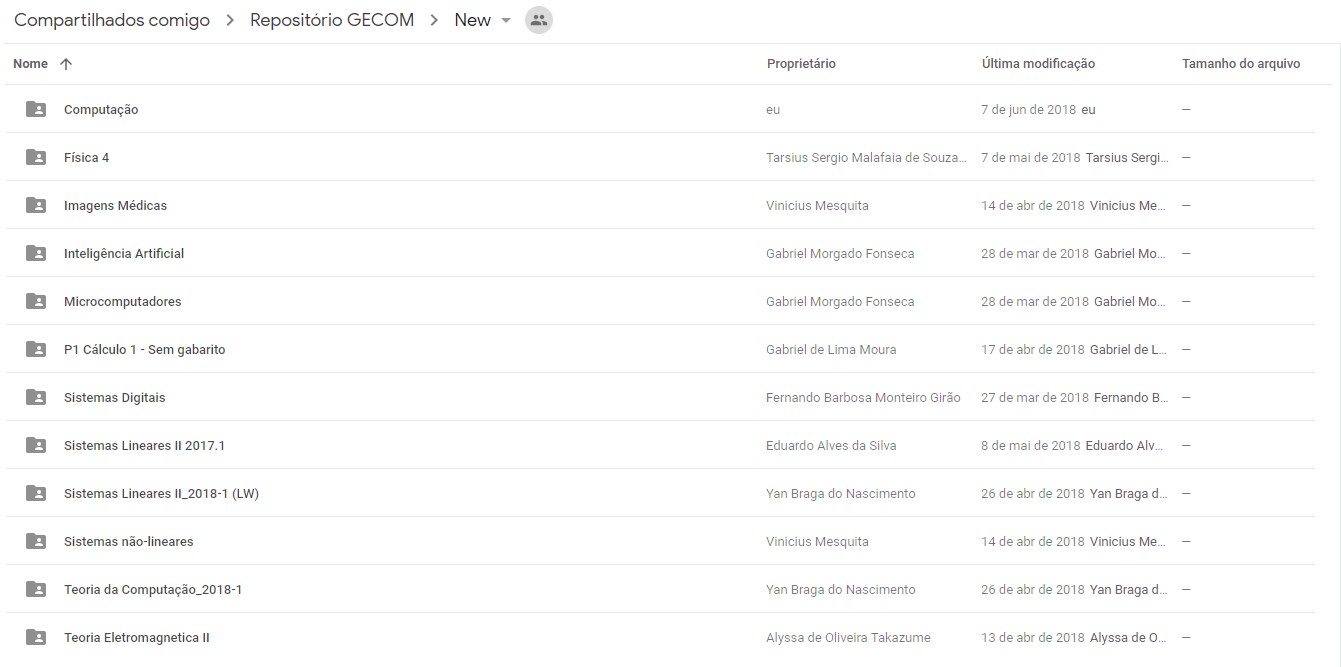
\includegraphics[width=\textwidth]{assets/driveGecomPastaNew.png}
     	\captionof{figure}{Diretórios já existente na pasta \textit{New} no momento do \textit{screenshot}}	
    \end{center}
    
    \begin{center}
    	3) Dentro do diretório da disciplina, verifique se o arquivo que você deseja upar não deve pertencer a uma sub-pasta da disciplina. Por exemplo, no caso da imagem a seguir, vemos que o aluno enviou uma P1 (Prova 1) e a colocou dentro de um diretório \textit{P1}. Tente sempre separar os arquivos da maneira mais lógica possível.

		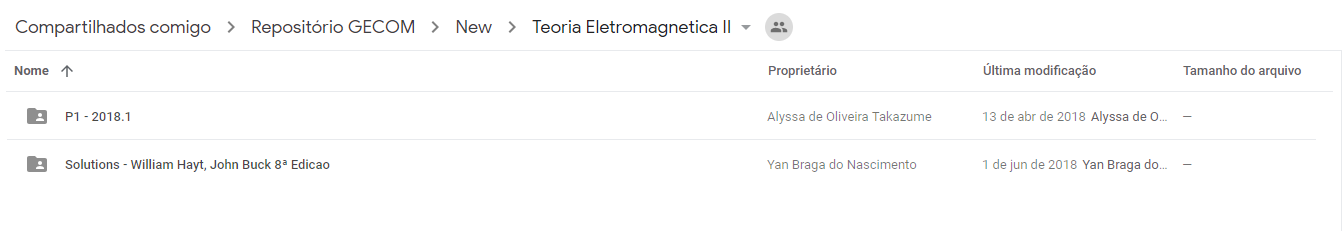
\includegraphics[width=\textwidth]{assets/driveGecomDiretorioP1.png}
     	\captionof{figure}{Aluno criou o diretório P1 - 2018.1 para upar a prova}
	
    \end{center}
    
    Depois de seguir esses passos, de tempos em tempos, membros do GECOM verificam esses arquivos e os transferem para a pasta definitiva \textit{Matérias}. Você, como aluno, não tem permissão para modificar o conteúdo da pasta \textit{Matérias}, por isso implementamos o sistema da pasta \textit{New}. Qualquer conteúdo que seja colocado como contribuição nessa pasta será antes avaliado segundo as autorizações que temos dos professores, para termos certeza de que o mesmo autorizou a divulgação do material, e, assim, evitar algum problema. 